\section{Preparando el espacio de trabajo}
Empezamos descargando la imagen ubuntu 20.04 de \href{https://hub.docker.com/\_/ubuntu}{Docker Hub}

\begin{figure}[H]
  \centering
  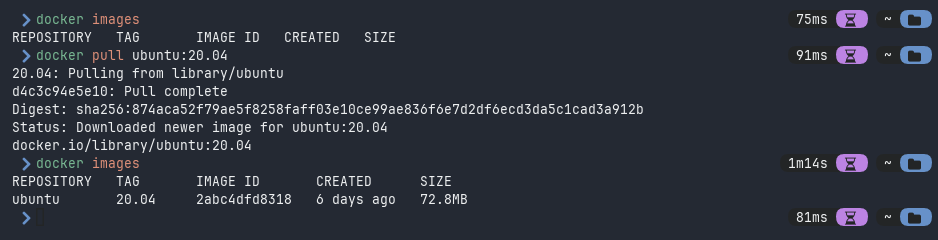
\includegraphics[width=1.0\textwidth]{img/ubuntu_image.png}
  \caption{Instalando la imagen ubuntu:20.04}
\end{figure}

Despues creamos un contenedor a partir de esta imagen y lo iniciamos inmediatamente. Podemos lograr estas 
acciones por separado usando los comandos \textcolor{blue}{docker create} y seguidamente \mininline{zsh}{docker start}. Sin embargo al no ejecutar ningún programa dentro del contenedor, este se detendrá inmediatamente. 
\singlespacing
Para el primer inicio del contenedor, podemos usar el comando \textcolor{blue}{docker run}, junto con otros 
opciones y argumentos:\\ 

\begin{itemize}
  \item Podemos establecer un nombre especifico al contenedor, si no hacemos esto, todas las operaciones que hagamos con el contenedor, tendremos que utilizar su hash generado. Al igual que Git con repositorios remotos. La opción es \textcolor{blue}{--name}
  \item Aprovechamos realizanso el \textbf{Port Mapping} de los puertos de la  maquina host a los puertos del contenedor usando la opcion \textcolor{blue}{-p}
  \item Interactuar con el contenedor con la opción \textcolor{blue}{-it} para que habra una terminal iterativa y dentro de la terminal  ejecutamos el inteprete de comandos de bash, el ejcutable es \textcolor{blue}{/bin/bash}
\end{itemize}

\begin{figure}[H]
  \centering
  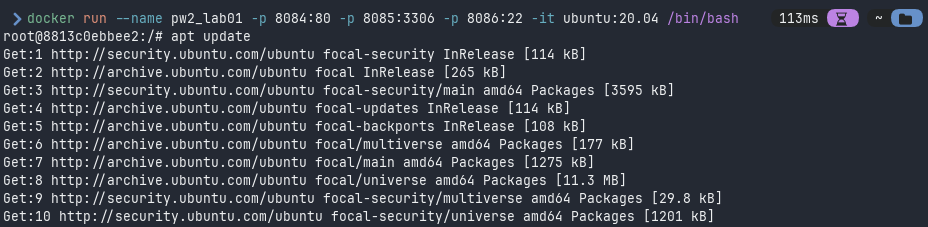
\includegraphics[width=1.0\textwidth]{img/run_container.png}
  \caption{Creando y ejecutando el contenedor}
\end{figure}

Ahora procedemos con la instalación de un editor de texto necesario para editar código (neovim), un servidor web que implemente el protocolo HTTP y HTTPS (Apache), unos lenguajes de scripting (perl, python), un sistema de gestion de base de datos (MariaDB) y finalmente un programa servidor que implemente el protocolo SSH (openssh)

\begin{figure}[H]
  \centering
  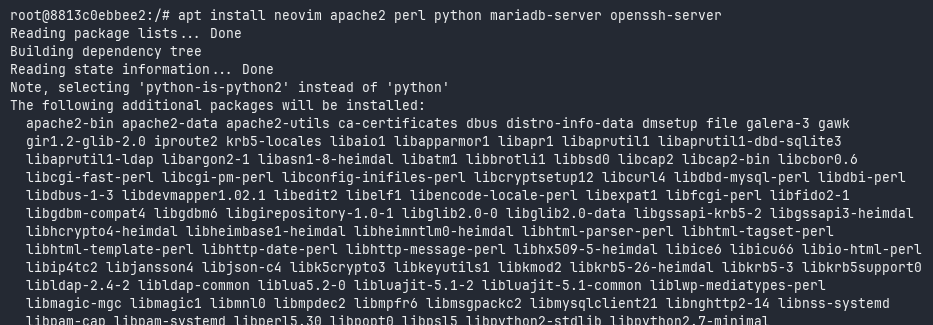
\includegraphics[width=1.0\textwidth]{img/install_programs.png}
  \caption{Instalando los programas para crear y administrar nuestro servidor web}
\end{figure}

Podemos verificar el estado de los programas servidor que hemos instalado. Estos servicios son conocidos como \textbf{Demonios} ya que son bucles infinitos que siempre estan escuchando. Los servidores siempre se 
deben de activar, incluso podemos configurar su habilitación  automatica cuando arranque el sistema operativo.

\begin{figure}[H]
  \centering
  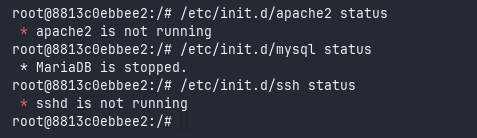
\includegraphics[width=0.6\textwidth]{img/check_daemons.png}
  \caption{Estado de los programas servidor}
\end{figure}

Por el momento solo vamos a iniciar el servidor web Apache y el sistema de gestion de base de datos MariaDB.

\begin{figure}[H]
  \centering
  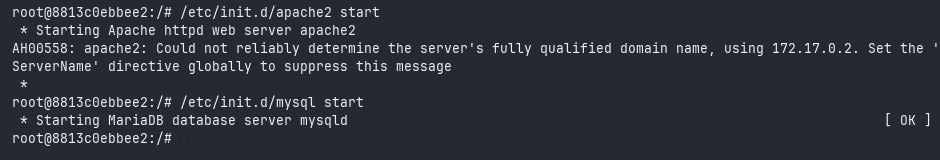
\includegraphics[width=1.0\textwidth]{img/start_daemons.png}
  \caption{Comenzar los demonios}
\end{figure}

Podemos probar el funcionamiento del servidor web de nuestro contenedor en nuestro navegador de nuestra 
maquina host poniendo la dirección IP del contenedor, o simplemente instalando y usando el programa 
\textcolor{blue}{curl} que es una herramienta en la terminal.

\begin{figure}[H]
  \centering
  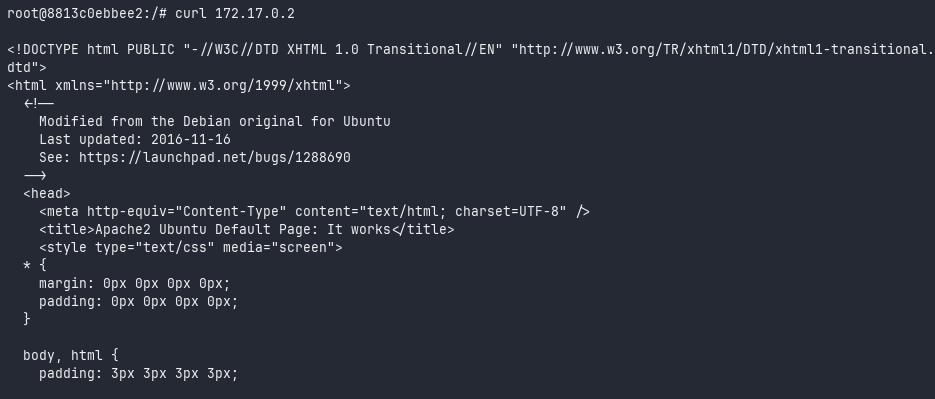
\includegraphics[width=1.0\textwidth]{img/server.png}
  \caption{Archivo \textit{index.html} ubicado en el directorio por defecto \textit{/var/www/html}}
\end{figure}

\subsection{Habilitando la ejecución de CGIs en Apache}
Apache trae consigo dos modulos nativos \textit{mod-cgi} y \textit{mod-cgid} y por defecto Apache solo escuha y ejecuta los scripts ubicados en el directorio especifico \textit{/usr/lib/cgi-bin}
\singlespacing
Vamos a crear un test en Python para ver el funcionamiento. Una vez que creamos el archivo .py, tenemos 
que otorgarle el permiso de ejecución, ya que es un script que Apache debe de ejecutar.

\begin{figure}[H]
  \centering
  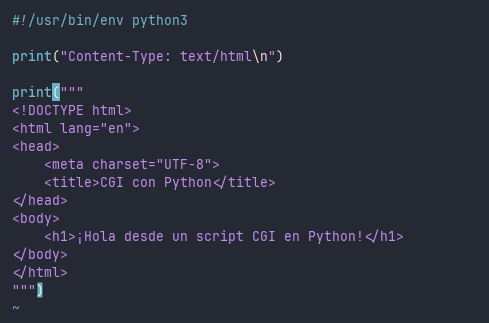
\includegraphics[width=0.5\textwidth]{img/create_cgi.png}
  \caption{Archivo en \textit{/usr/lib/cgi-bin/test.py}}
\end{figure}

\begin{figure}[H]
  \centering
  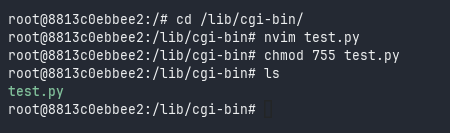
\includegraphics[width=0.6\textwidth]{img/cgi_with_python.png}
  \caption{Estableciendo permisos de ejecución}
\end{figure}

Si intentamos ejecutar el script, Apache ni intentará buscarlos porque hasta el momento solo escuha en el directorio \textit{/var/www/html}
\begin{figure}[H]
  \centering
  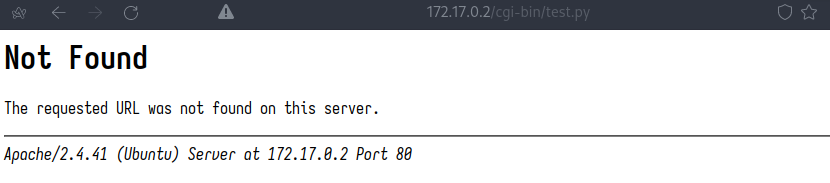
\includegraphics[width=1.0\textwidth]{img/test_error.png}
  \caption{Apache no escucha en este directorio}
\end{figure}

Pasa que alta hacer alguna configuracion para que Apache pueda realizar esta funcionalidad. Nosotros debemos de habilitar los modulos CGI. Una vez activados los modulos, debemos de reiniciar Apache para que las configuraciones sean leidas.

\begin{figure}[H]
  \centering
  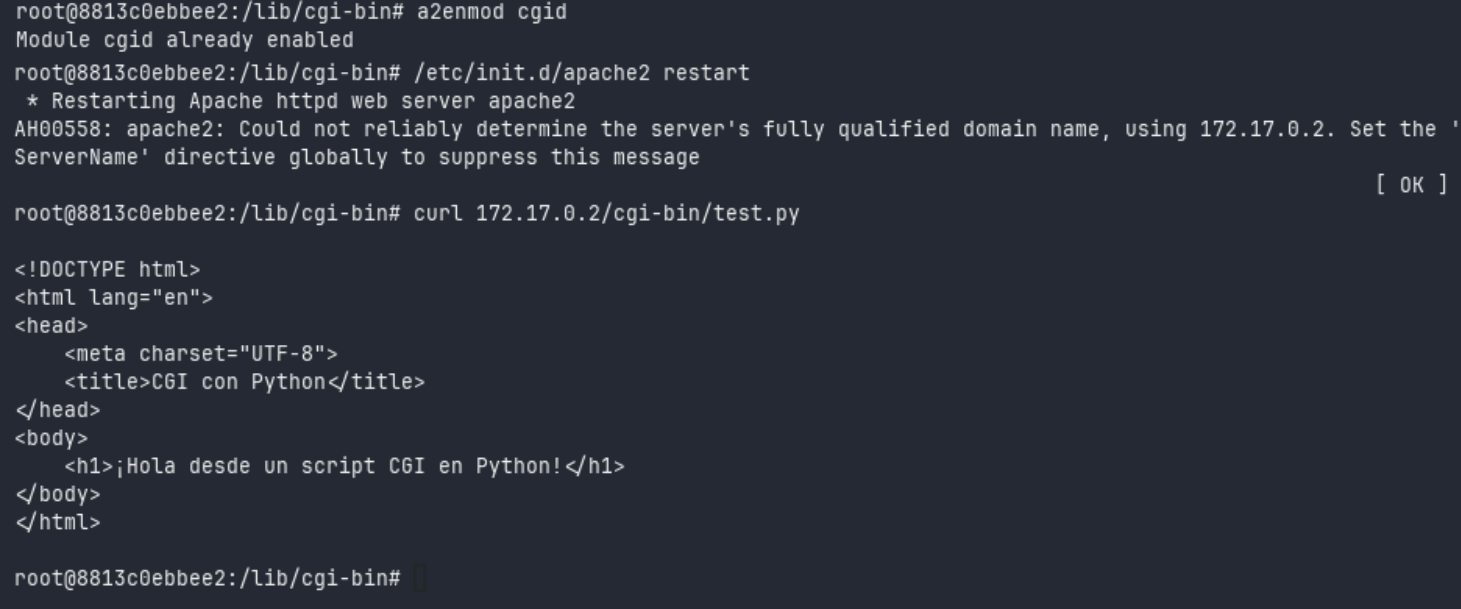
\includegraphics[width=1.0\textwidth]{img/restart.png}
  \caption{Activar los modulos, reiniciar el servidor y probar}
\end{figure}

Ahora si podemos estar seguros que los CGIs se van a ejecutar, tambien podemos probarlo desde el navegador de la maquina host

\begin{figure}[H]
  \centering
  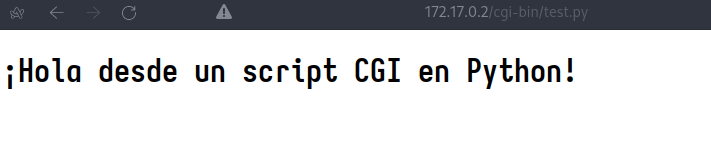
\includegraphics[width=0.8\textwidth]{img/test.png}
  \caption{Test exitoso}
\end{figure}

\subsection{Cambiando a directorios personalizados}
Para hacer los cambios, nosotros debemos modificar los archivos de configuración de apache. Apache 
maneja el concepto de \textbf{Virtual Host} que nos permite tener varias aplicaciones web en solo un servidor 
web fisico. Esto se logra configurando Apache para que responda a diferentes nombres de dominio (o direcciones IP) y sirva contenido específico para cada uno de ellos.\\

\subsubsection{Ejemplo con el directorio raiz /aplicaciones\_web que almacena la aplicacion web proyecto-final-pweb1}

Las bloques de configuracion que vamos a realizar van a definir el nombre de dominio, el directorio raiz y 
otras opciones de configuracion. Vamos a crear un archivo \textit{/etc/apache2/sites-available/aplicaciones\_web} y aqui colocamos nuestras configuraciones.

\begin{figure}[H]
  \centering
  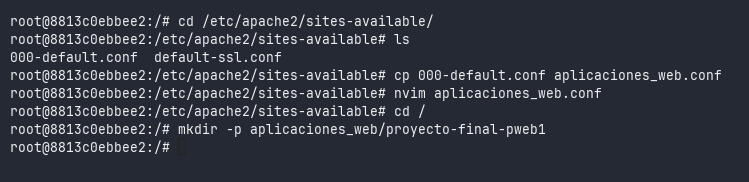
\includegraphics[width=0.8\textwidth]{img/directories.png}
  \caption{Creación del archivo de configuración}
\end{figure}

Es muy importante el uso de \textbf{ScriptAlias} porque nos permite organizar todos los scripts de la aplicación en un solo directorio especifico, el cual es el unico directorio que Apache busca los scripts y los va a ejecutar.

\begin{figure}[H]
  \centering
  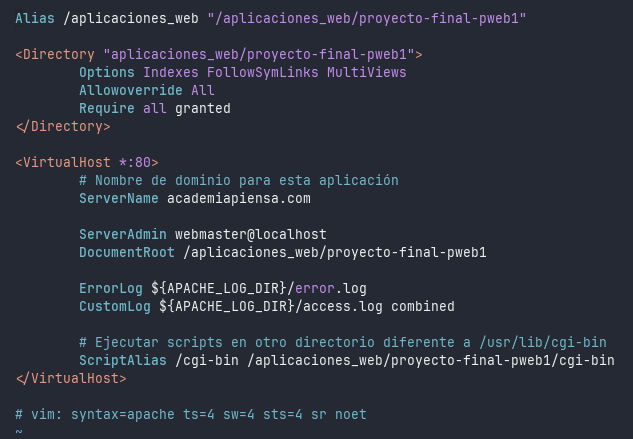
\includegraphics[width=0.6\textwidth]{img/conf.png}
  \caption{Configuración del Virtual Host}
\end{figure}

Una vez que hicimos las respectivas configuraciones, ahora necesitamos activar el sitio web y activar el modulo \textbf{mod-rewrite} que se encarga de realizar las redirecciones de solicitudes.

\begin{figure}[H]
  \centering
  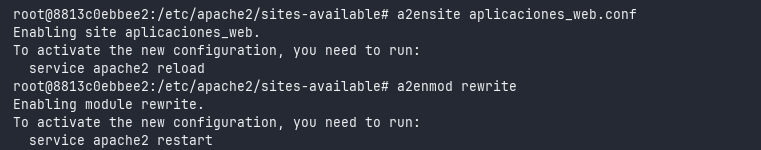
\includegraphics[width=0.8\textwidth]{img/enable_conf.png}
  \caption{Habilitamos el sitio web configurado}
\end{figure}

Por ultimo habilitamos la configuración que basicamente consiste en crear un enlace simbólico desde el archivo de configuración \textit{/etc/apache2/sites-available/aplicaciones\_web} al archivo correspondiente en \textit{/etc/apache2/sites-enabled/aplicaciones\_web}.\\
Para que las configuraciones se establezcan, reiniciamos el servidor Apache.

\begin{figure}[H]
  \centering
  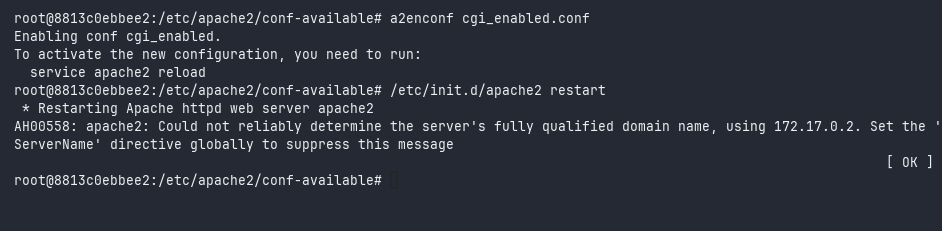
\includegraphics[width=1.0\textwidth]{img/restart2.png}
  \caption{Habilitando las configuración}
\end{figure}

\subsection{Agregando un usuario para que pueda controlar el sitio web creado}
Podemos agegar a un usuario para que se encargue de  administrar este sitio web. Entonces lo primero 
que haremos es crear el usuario en el sistema y después cambiaremos el propietario y el grupo del directorio 
raiz \textit{/aplicaciones\_web} y todos los directorios y archivos dentro de este.

\begin{figure}[H]
  \centering
  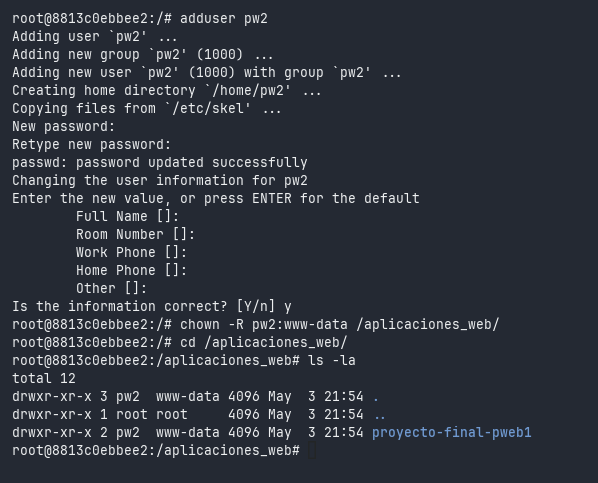
\includegraphics[width=0.6\textwidth]{img/adduser.png}
  \caption{Agregado un usuario y cambiando propietario}
\end{figure}

Ahora podemos probar el servicio SSH, para ello lo vamos a activar y nos conectaremos desde la maquina host

\begin{figure}[H]
  \centering
  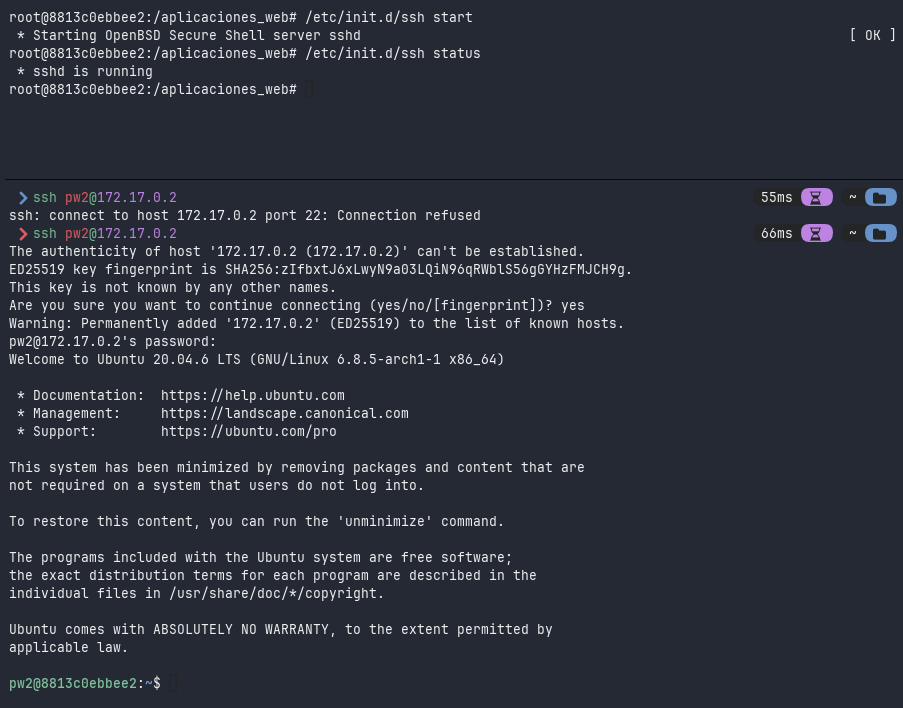
\includegraphics[width=1.0\textwidth]{img/ssh.png}
  \caption{El servicio de SSH esta habilitado}
\end{figure}


